% Generated by tools/build_report.py from this template and executed results/*.csv.
\documentclass{article}
\PassOptionsToPackage{numbers,compress}{natbib}
\usepackage[main,final]{neurips_2026}
\makeatletter
\renewcommand{\@noticestring}{DSAA2011 Machine Learning, Course Project (Task A), HKUST(GZ), Fall 2026.}
\makeatother
\usepackage[utf8]{inputenc}
\usepackage[T1]{fontenc}
\usepackage{hyperref,url,booktabs,amsmath,amsfonts,graphicx,microtype,xcolor,placeins}
\renewcommand{\ttdefault}{lmtt}
\graphicspath{{../figures/}}
\title{``Where am I?'' Identifying Australia's Climate Zone\\from Daily Weather Observations}
\author{Group XX\\DSAA2011 (L02), HKUST(GZ)\\\texttt{Member A, Member B, Member C, Member D}}
@@MACROS@@
\begin{document}
\maketitle
\begin{abstract}
We ask how much information about a station's climate zone is contained in a day of weather, and how this changes when past observations are available. We annotate Rain in Australia with five project-defined groups of K\"oppen--Geiger codes, retaining 142,451 daily records from 48 stations. t-SNE and clustering describe local weather structure; supervised models predict the externally assigned climate labels. We distinguish new days at known stations from withheld stations in this network. A revised, class-covered four-fold protocol nests parameter, window and feature selection inside training stations. Across nine daily configurations, \BestDailyName\ has the highest primary pooled five-class macro-F1 (\BestDailyScore); this ranking is descriptive. The predefined histogram gradient-boosted tree (HGB) reference obtains \DailyHGB, and its inner-selected history-window procedure obtains \SelectedWindow. Repeated partitions and station-level resampling describe sensitivity, but do not constitute external validation. The conclusions concern this network and one raster annotation, with no claim of uniquely optimal windows or causal attribution of protocol gaps.
\end{abstract}

\section{Introduction}
A day of weather and a climate classification describe different time scales. K\"oppen classes depend on long-term temperature and precipitation statistics; a single observation need not identify them. Using the supplied Rain in Australia dataset \citep{kaggle}, we study a five-class target rather than its usual \texttt{RainTomorrow} label. The project connects three questions: what structure is visible without fitting a classifier, how much can daily measurements predict, and whether additional history helps more than additional model flexibility.

This is a retrospective information-recovery experiment. If coordinates and a climate map are already available, map lookup is simpler than weather-based classification. Our intended test is the information available in weather when the map label is withheld, not a geographical localisation service. A withheld station here is drawn from the existing 48-station network, not an arbitrary new Australian location.

The first version guided this revised protocol. All experiments were rerun with new caches and training-only selection, but earlier exploration cannot be undone: this is not a preregistered study or an independent external confirmation. We preserve the task and explicitly narrow unsupported claims.

\section{Mandatory tasks}
\subsection{Target construction and preprocessing}
Each dataset \texttt{Location} is manually matched to a Bureau of Meteorology station number and coordinate \citep{bom}. \texttt{kgcpy} 1.1.8 assigns a code from its 100-arc-second raster \citep{kgc,rubel,map}. Our groups are Tropical (observed Am/Aw), Arid (BWh/BSh/BSk), Subtropical (Cfa), Mediterranean (Csa/Csb), and Oceanic (Cfb). This mixes whole A/B groups with subdivisions of C to obtain interpretable classes represented in the supplied data. The complete mapping and neighbouring-pixel codes are provided in \texttt{data/processed/location\_zone.csv} and the notebook. Manual matching and the 1986--2010 raster reference period introduce annotation uncertainty.

Norfolk Island receives an ocean code and is excluded, leaving 48 stations. Tropical has only four stations; Arid has seven. Rows are imbalanced (7.6--32.2\% per class), so the primary metric weights classes equally. The majority accuracy is 0.322; this is not a macro-F1 baseline. Station count, rather than the number of correlated days, limits evidence for transfer.

\texttt{Location}, future \texttt{RainTomorrow}, and any \texttt{RISK\_MM} are excluded from predictors. Station IDs are used only for splits, within-station histories and diagnostics. Wind speeds/directions become six vector components, $(u,v)=(-s\sin\theta,-s\cos\theta)$; calm wind is $(0,0)$. Three speeds are also retained. Rainfall uses $\log(1+x)$, and redundant \texttt{RainToday} is dropped. Day-of-year sine/cosine encode season; year is excluded. The retained core contains 20 features. Median imputation and scaling are fitted within each training fold. HGB uses median imputation without scaling.

Missingness is concentrated by station. A missing-flag-only tree provides an exploratory diagnostic of station information, but does not prove that all such information is non-climatic. The core policy excludes Sunshine, Evaporation and Cloud9am/3pm, and has no explicit missing indicators. This policy originated in earlier exploration; it is fixed for the new run and compared with full-feature policies in an outer-fold sensitivity check. Median values may themselves carry missingness information, so we do not claim to eliminate every station cue.

\subsection{t-SNE visualization}
We sample 1,200 days per class (6,000 total), impute/standardise, and fit t-SNE \citep{tsne} with perplexity 30, PCA initialisation and seed 42. Labels determine balanced sampling but do not enter embedding optimisation. Other perplexities (5/50/100), seeds (0/7), season-restricted subsets and a no-calendar-feature embedding are checked in the notebook. These are exploratory views of a reweighted population.


\begin{figure}[htbp]\centering
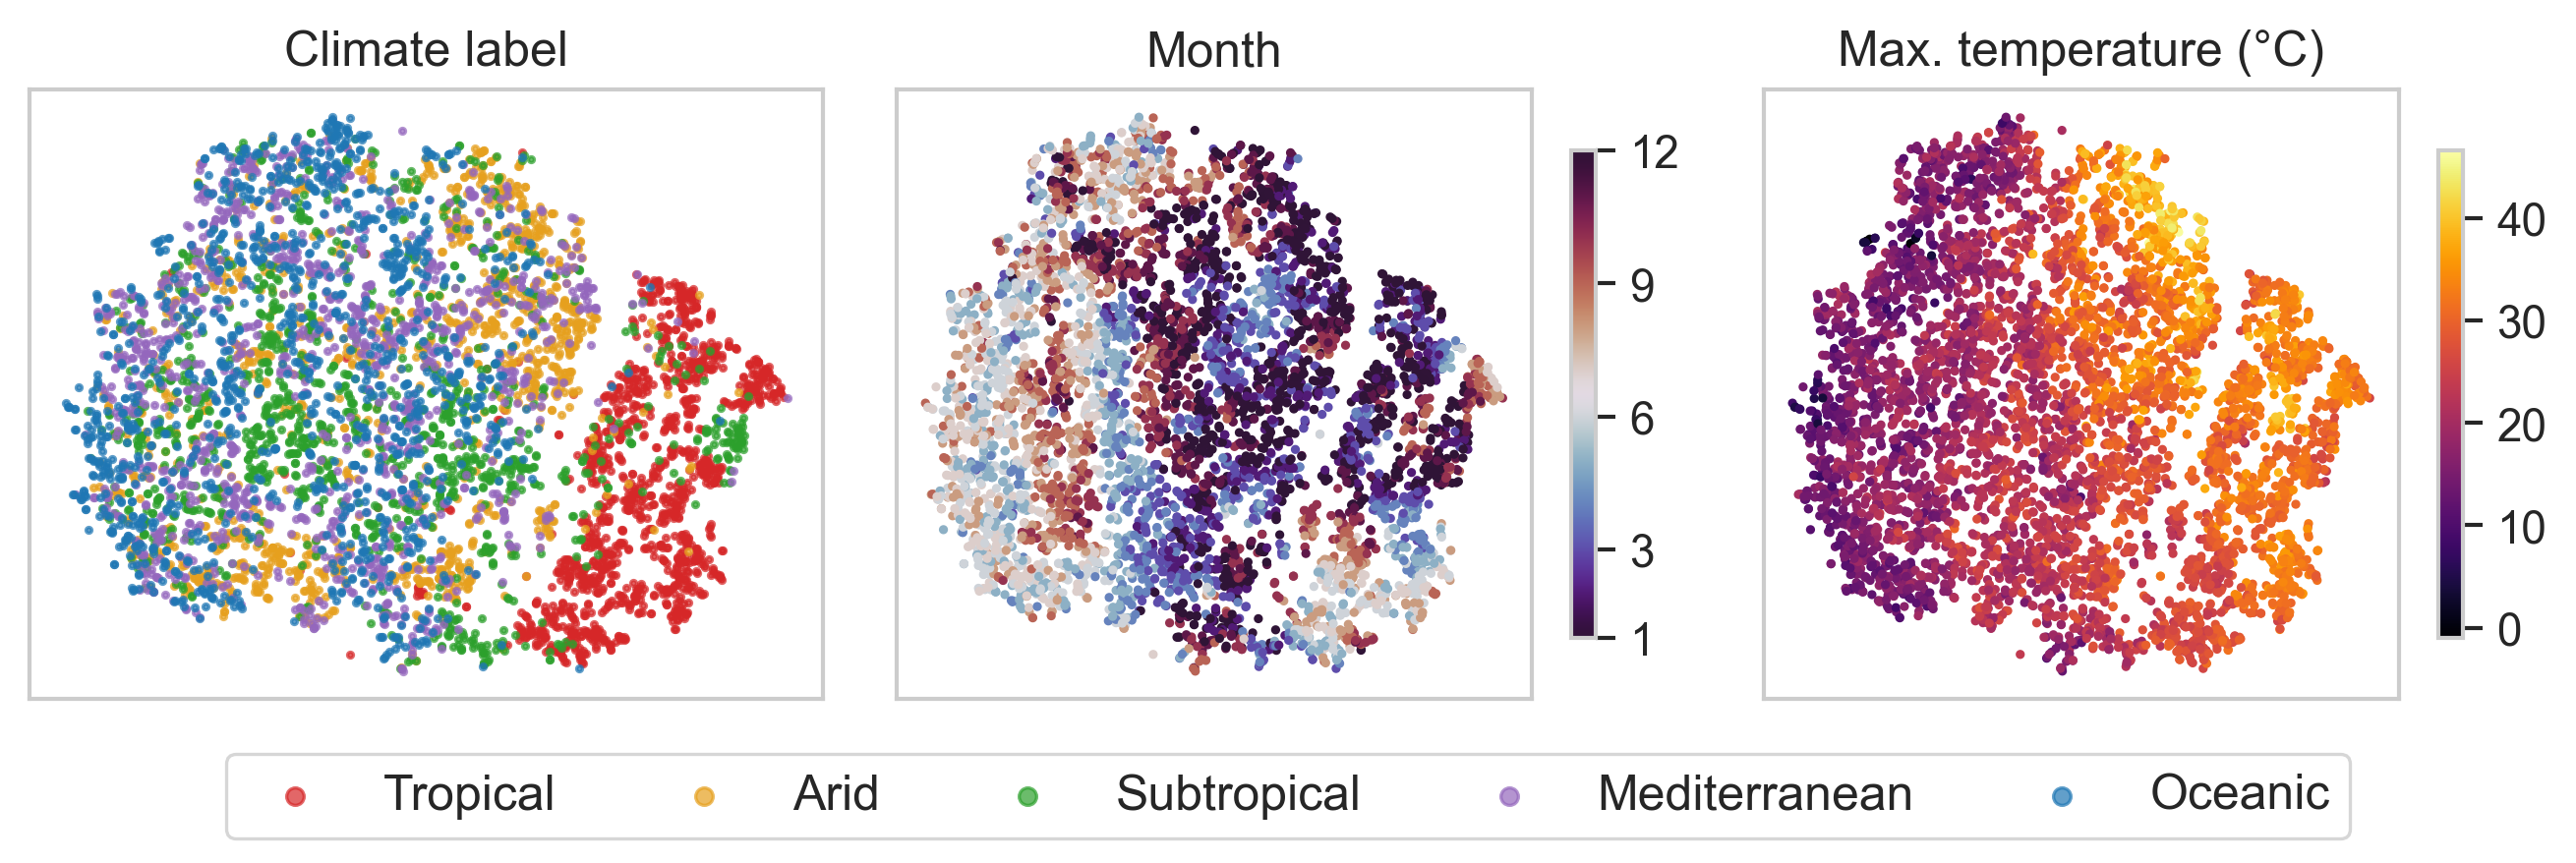
\includegraphics[width=\linewidth]{report_tsne}
\caption{Same t-SNE embedding coloured by climate group, month and maximum temperature. Labels influence sampling, not optimisation.}\label{fig:tsne}
\end{figure}

The two-dimensional t-SNE trustworthiness is \TsneTrust\ versus \PcaTrust\ for two-component PCA; diagnostic 10-NN zone classification accuracy is \TsnePurity. These scores describe local neighbourhoods after using all points in the embedding. They are not held-out generalisation estimates: days from the same station occur in multiple diagnostic folds. Cohen's kappa adjusts chance agreement but is not a common information scale for season, zone and station prediction. Apparent islands, sizes and inter-island distances should not be read as physical climate distances. The classification experiments use the original features, not t-SNE coordinates.

\subsection{Clustering}
K-means, Ward agglomeration and full-covariance Gaussian mixtures are fitted in the 20-dimensional space for $k=2,\ldots,10$. They represent centroid, hierarchical and probabilistic approaches. We report silhouette \citep{sil}, Davies--Bouldin, Calinski--Harabasz, inertia/BIC and agreement with climate labels (ARI \citep{ari}, NMI). NMI is not chance-adjusted. Refit stability compares labels on shared points after ten 80\% day subsamples.

The inherited descriptive rule ranks the three compactness metrics and requires stability at least 0.90. It was devised after the earlier analysis, not prospectively validated. Its selected partition is \ClusterChoice; Table~\ref{tab:cluster} compares algorithms at $k=3$. The absolute silhouette remains small even for stable solutions: repeatability does not establish well-separated natural classes. Varying thresholds (0.80--0.95) retains $k=3$ when Davies--Bouldin is included, but using silhouette and Calinski--Harabasz alone selects $k=2$. The rule is therefore not uniquely supported. Natural-frequency sampling and whole-station/year perturbations are also reported. GMM covariance-floor and convergence diagnostics test sensitivity to point masses from dry days and imputation; numerical convergence does not imply physical suitability.

@@CLUSTER_TABLE@@
K-means agreement with the reference partition ranges from \StationClusterStability\ under whole-station perturbations and \YearClusterStability\ under whole-year perturbations. Its natural-frequency sample has climate-label ARI \NaturalClusterARI. Thus a reasonably repeatable daily partition can still recover little of the climate taxonomy; balancing by climate label also changes the population being described.

\begin{figure}[htbp]\centering
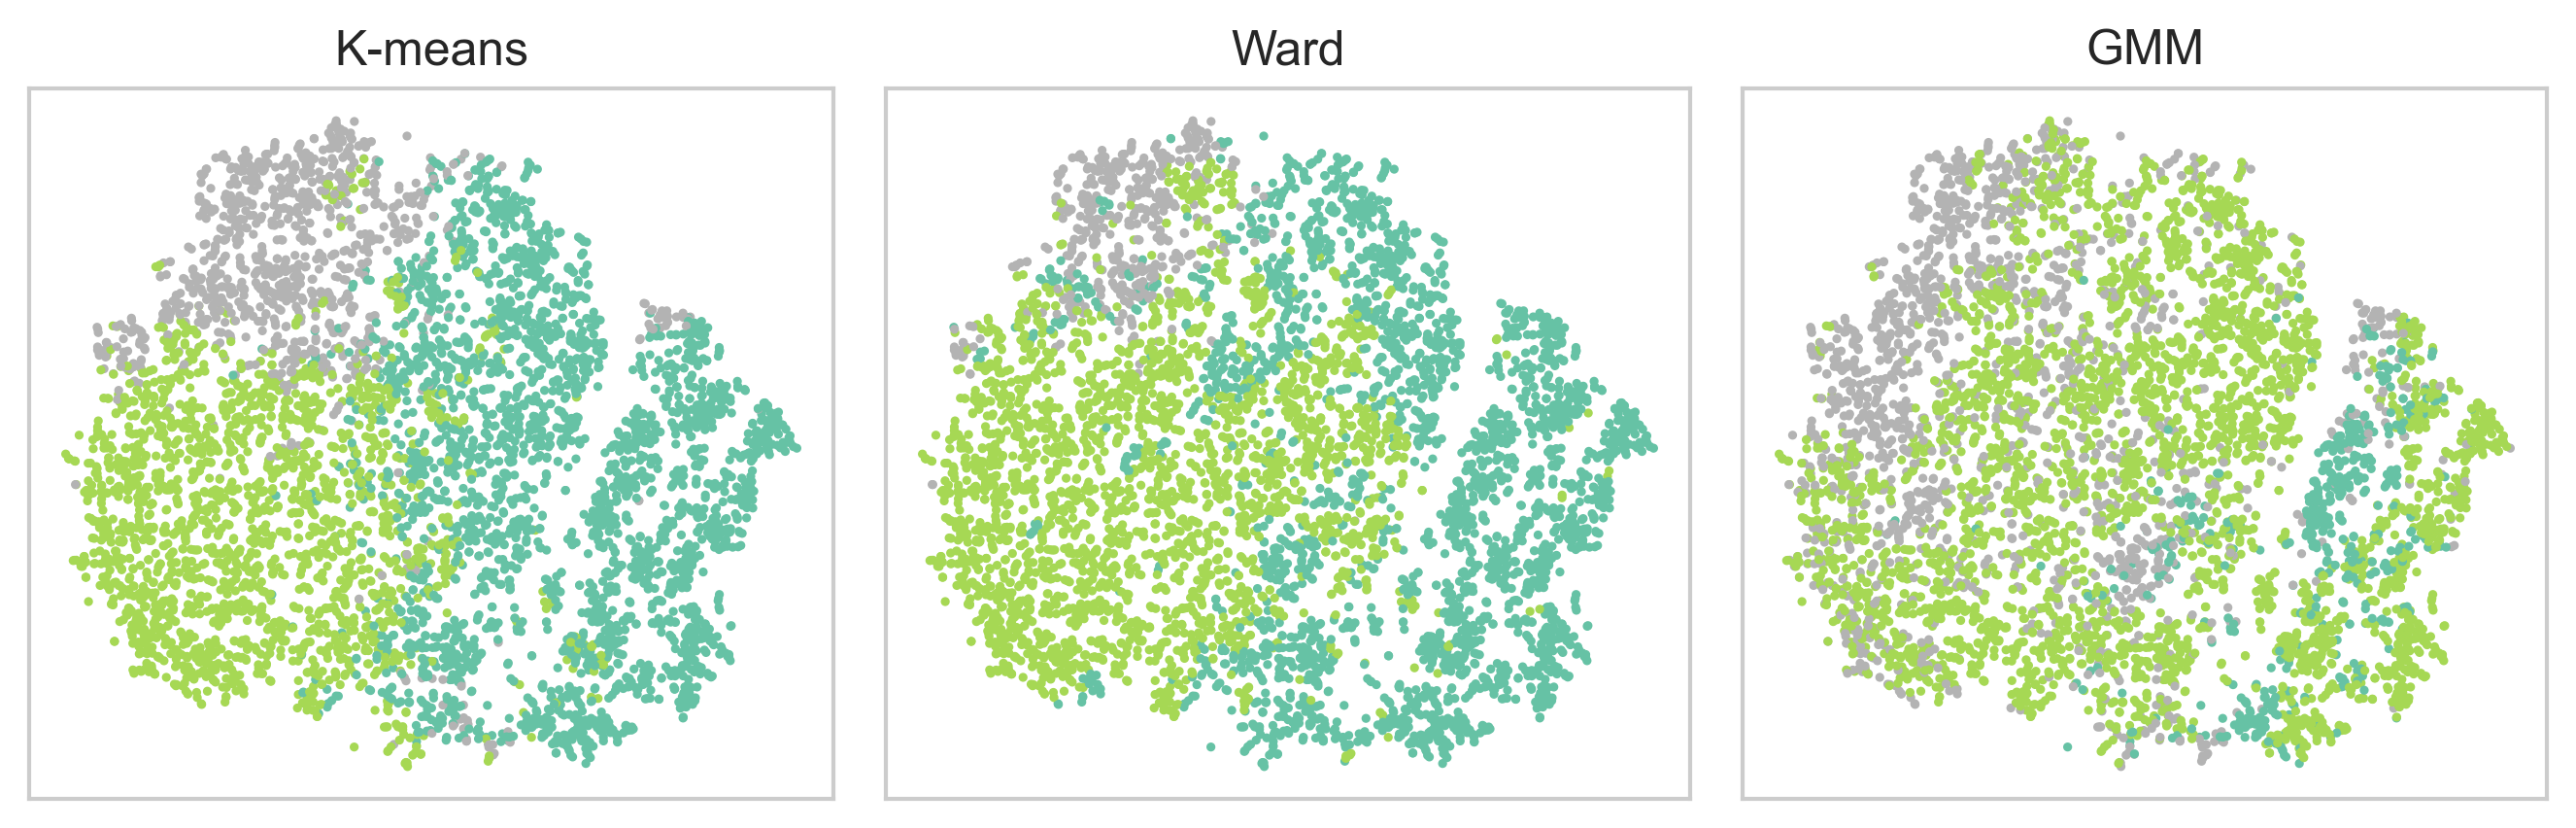
\includegraphics[width=\linewidth]{report_clusters}
\caption{Cluster assignments shown on t-SNE; colours are algorithm-specific cluster IDs. Clustering uses the original 20-dimensional representation.}\label{fig:clusters}
\end{figure}

Profiles support descriptive labels such as warm, cool with weaker winds, and cool with stronger winds and more rain. Synoptic fronts are a possible interpretation, not independently verified events. As a separate exercise, 48 station profiles (12 monthly means of four variables) are clustered by Ward at $k=5$, giving ARI \StationARI. This comparison changes the unit, representation, sample size and cluster count; its difference from daily ARI cannot isolate the effect of temporal averaging. A recovered coastal subset is not an entire climate class.

\subsection{Prediction: training, test and entire sets}
Multinomial logistic regression (LR) supplies a linear classifier with softmax probabilities; a default CART decision tree (DT) supplies a flexible nonlinear contrast. Both fit the core features. The course illustration uses stratified random 70/30 rows; a historical 70/30 station split gives an additional contrast. The latter is 70/30 in stations, not necessarily rows. Both splits were examined in earlier development and are not fresh holdouts. Table~\ref{tab:basic} reports train/test/entire scores; Fig.~\ref{fig:cm} shows the required confusion matrices.

@@BASIC_TABLE@@

\begin{figure}[htbp]\centering
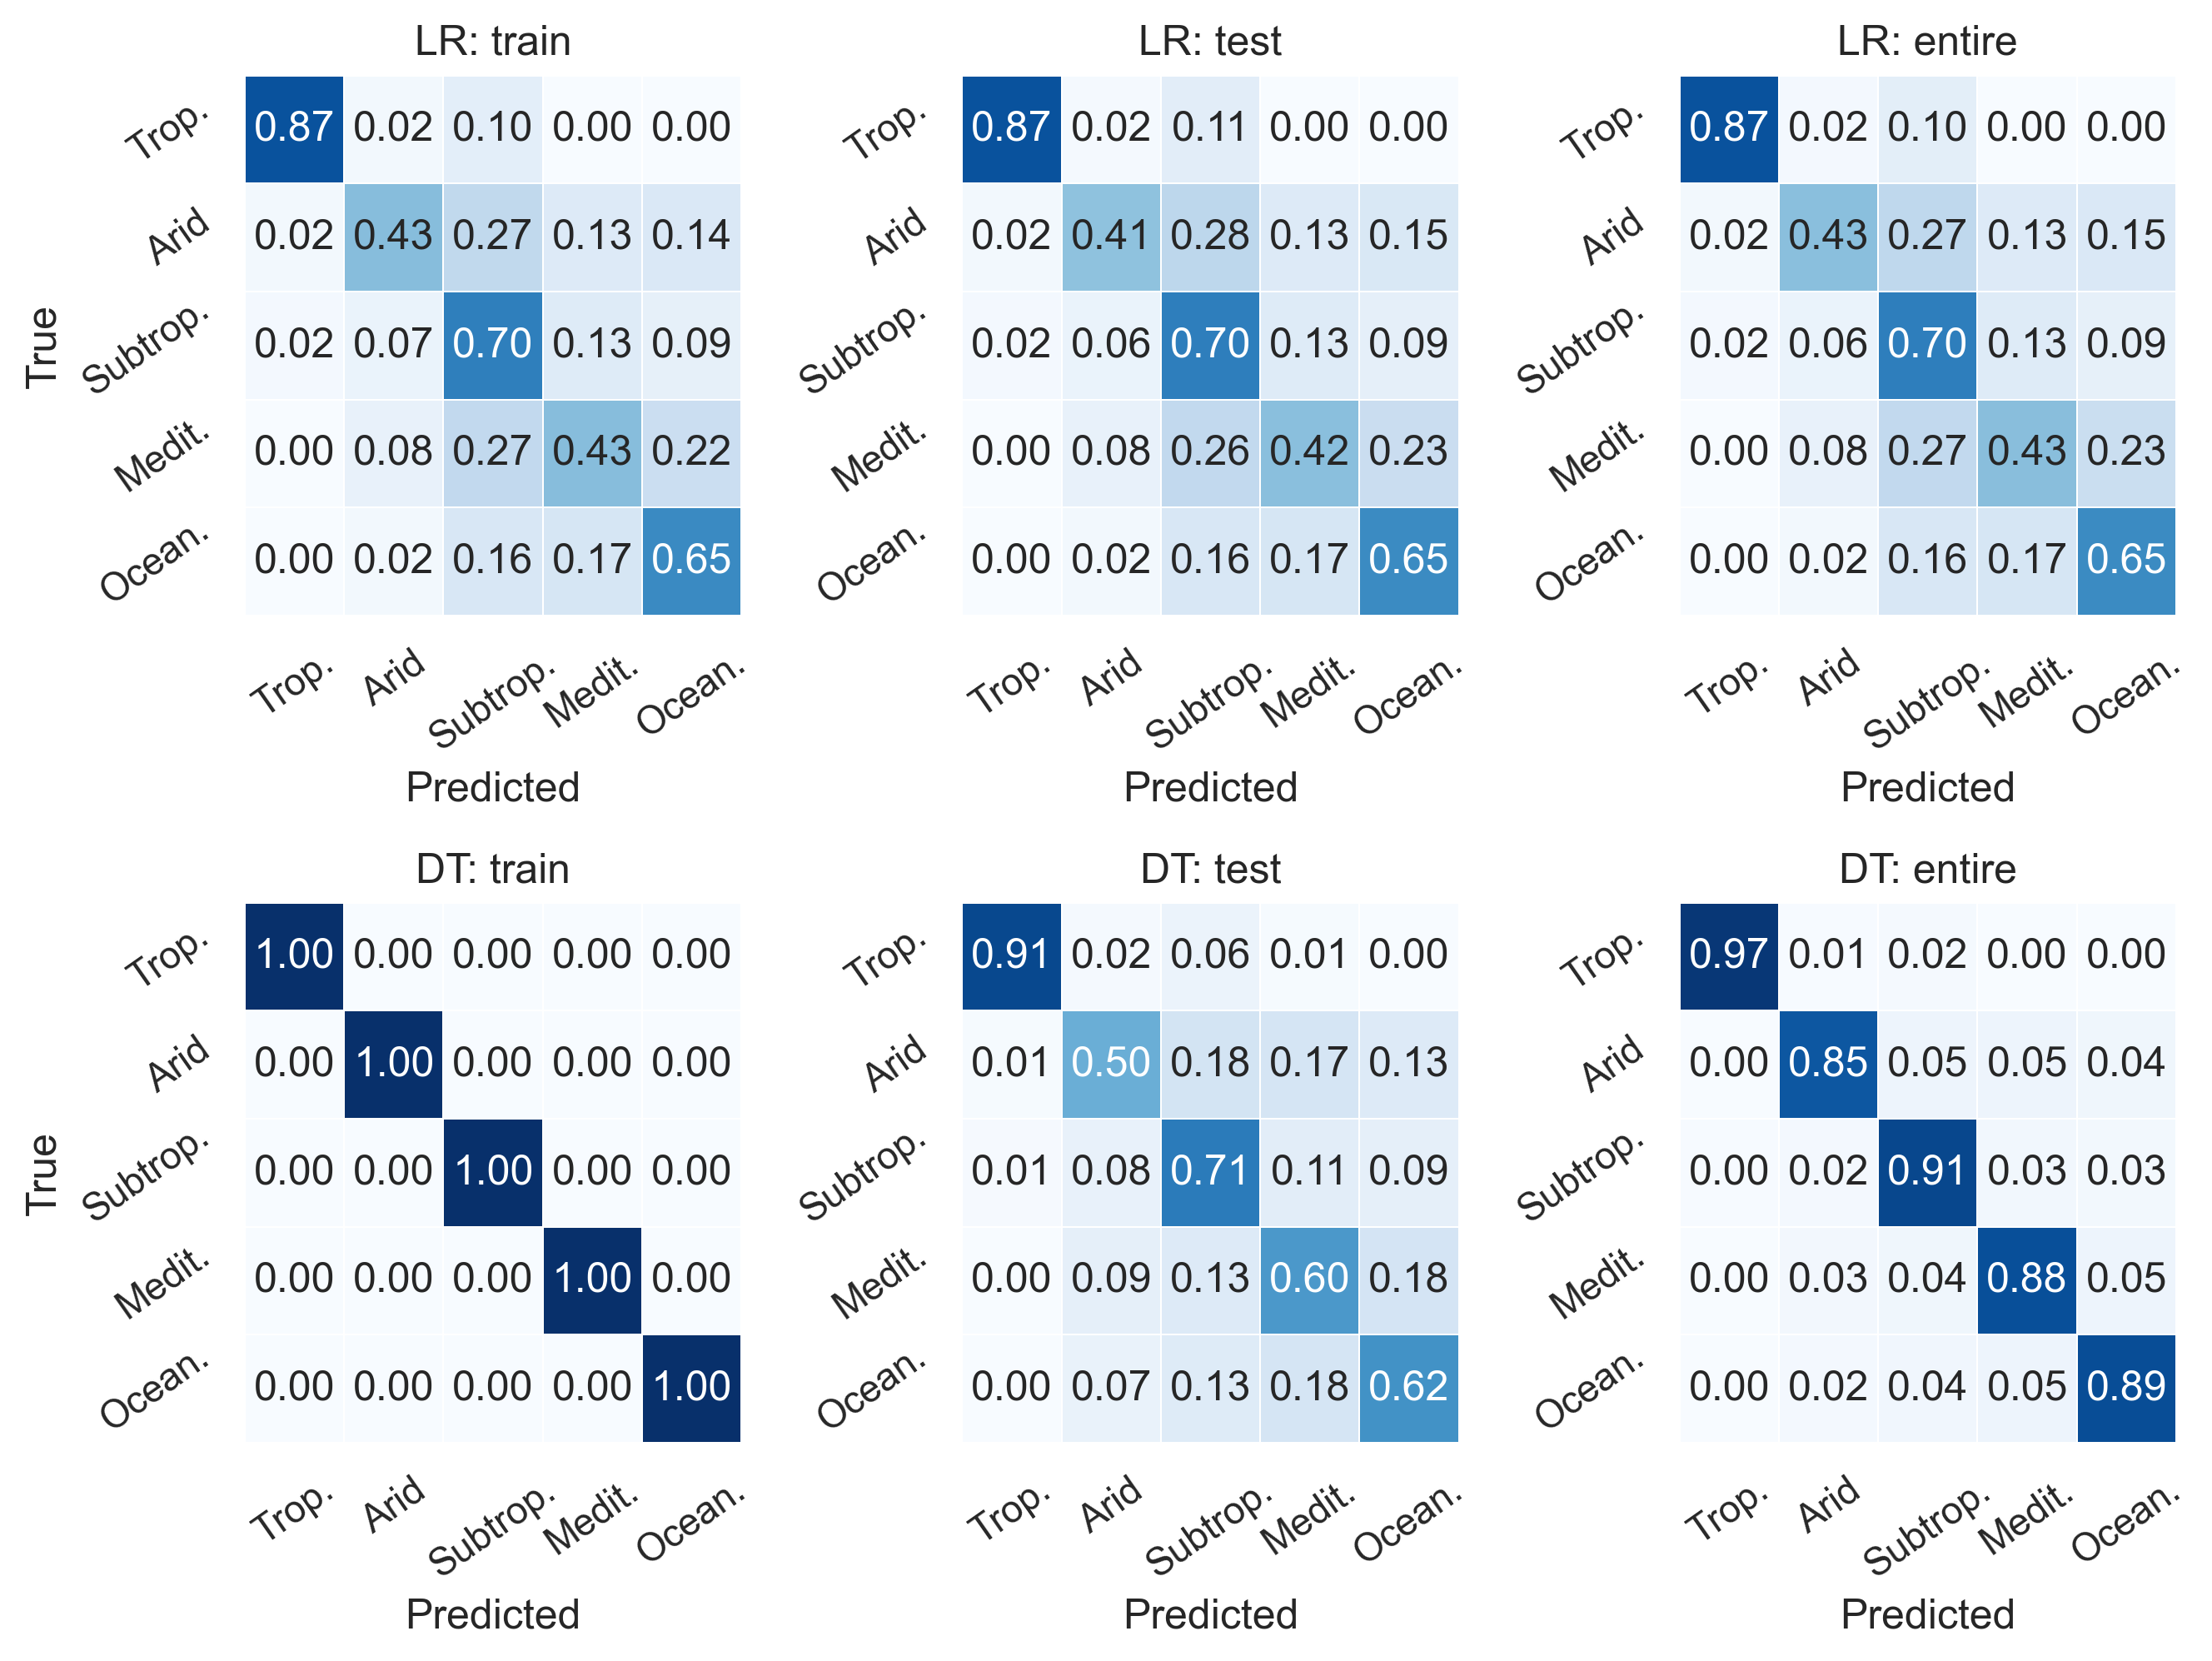
\includegraphics[width=.97\linewidth]{report_confusion}
\caption{Default LR and tree: random-split training, test and entire-set confusion matrices. Values and colour show row-normalised recall. Exact counts are in the notebook and exported CSV.}\label{fig:cm}
\end{figure}

Entire-set accuracy is a row-count-weighted average of train/test accuracy; macro-F1 is nonlinear and is recomputed from pooled predictions. Neither entire-set score is independent evidence of generalisation. A large tree gap indicates overfitting under this protocol. Similar LR train/test scores are consistent with limited flexibility, but do not prove that all error is bias or that 105 fitted coefficients cannot overfit correlated observations.

The notebook also retrains illustrative two-feature models on MinTemp and Humidity3pm. This pair was selected during earlier exploration, including test comparisons; its displayed boundaries are illustrative, not an independently validated feature-selection result. Final model decisions use all core features and the nested protocol below.

\subsection{Validation, metrics and model assessment}
Per-class precision, recall and F1 are calculated from the confusion matrices and checked against scikit-learn \citep{sklearn}. ROC/AUC is one-versus-rest using probabilities (Fig.~\ref{fig:roc}); macro-AUC averages the five binary AUCs. A default tree's nearly discrete leaf probabilities can produce a different AUC ordering from its hard-label accuracy. Complete per-class tables and validation curves are in the executed notebook and exported CSVs.

@@TUNING_TABLE@@
Table~\ref{tab:tuning} shows how validation changes each simple model. LR searches $C\in\{0.01,1,100\}$ and unweighted/balanced classes; the tree searches depth $\{4,8,16,\mathrm{unlimited}\}$ and minimum leaf sizes $\{5,20,100\}$. The selected settings need not improve every held-out score: validation is an estimate, not a guarantee. A nonzero minimum leaf size can regularise even when the selected depth is unlimited.


\begin{figure}[htbp]\centering
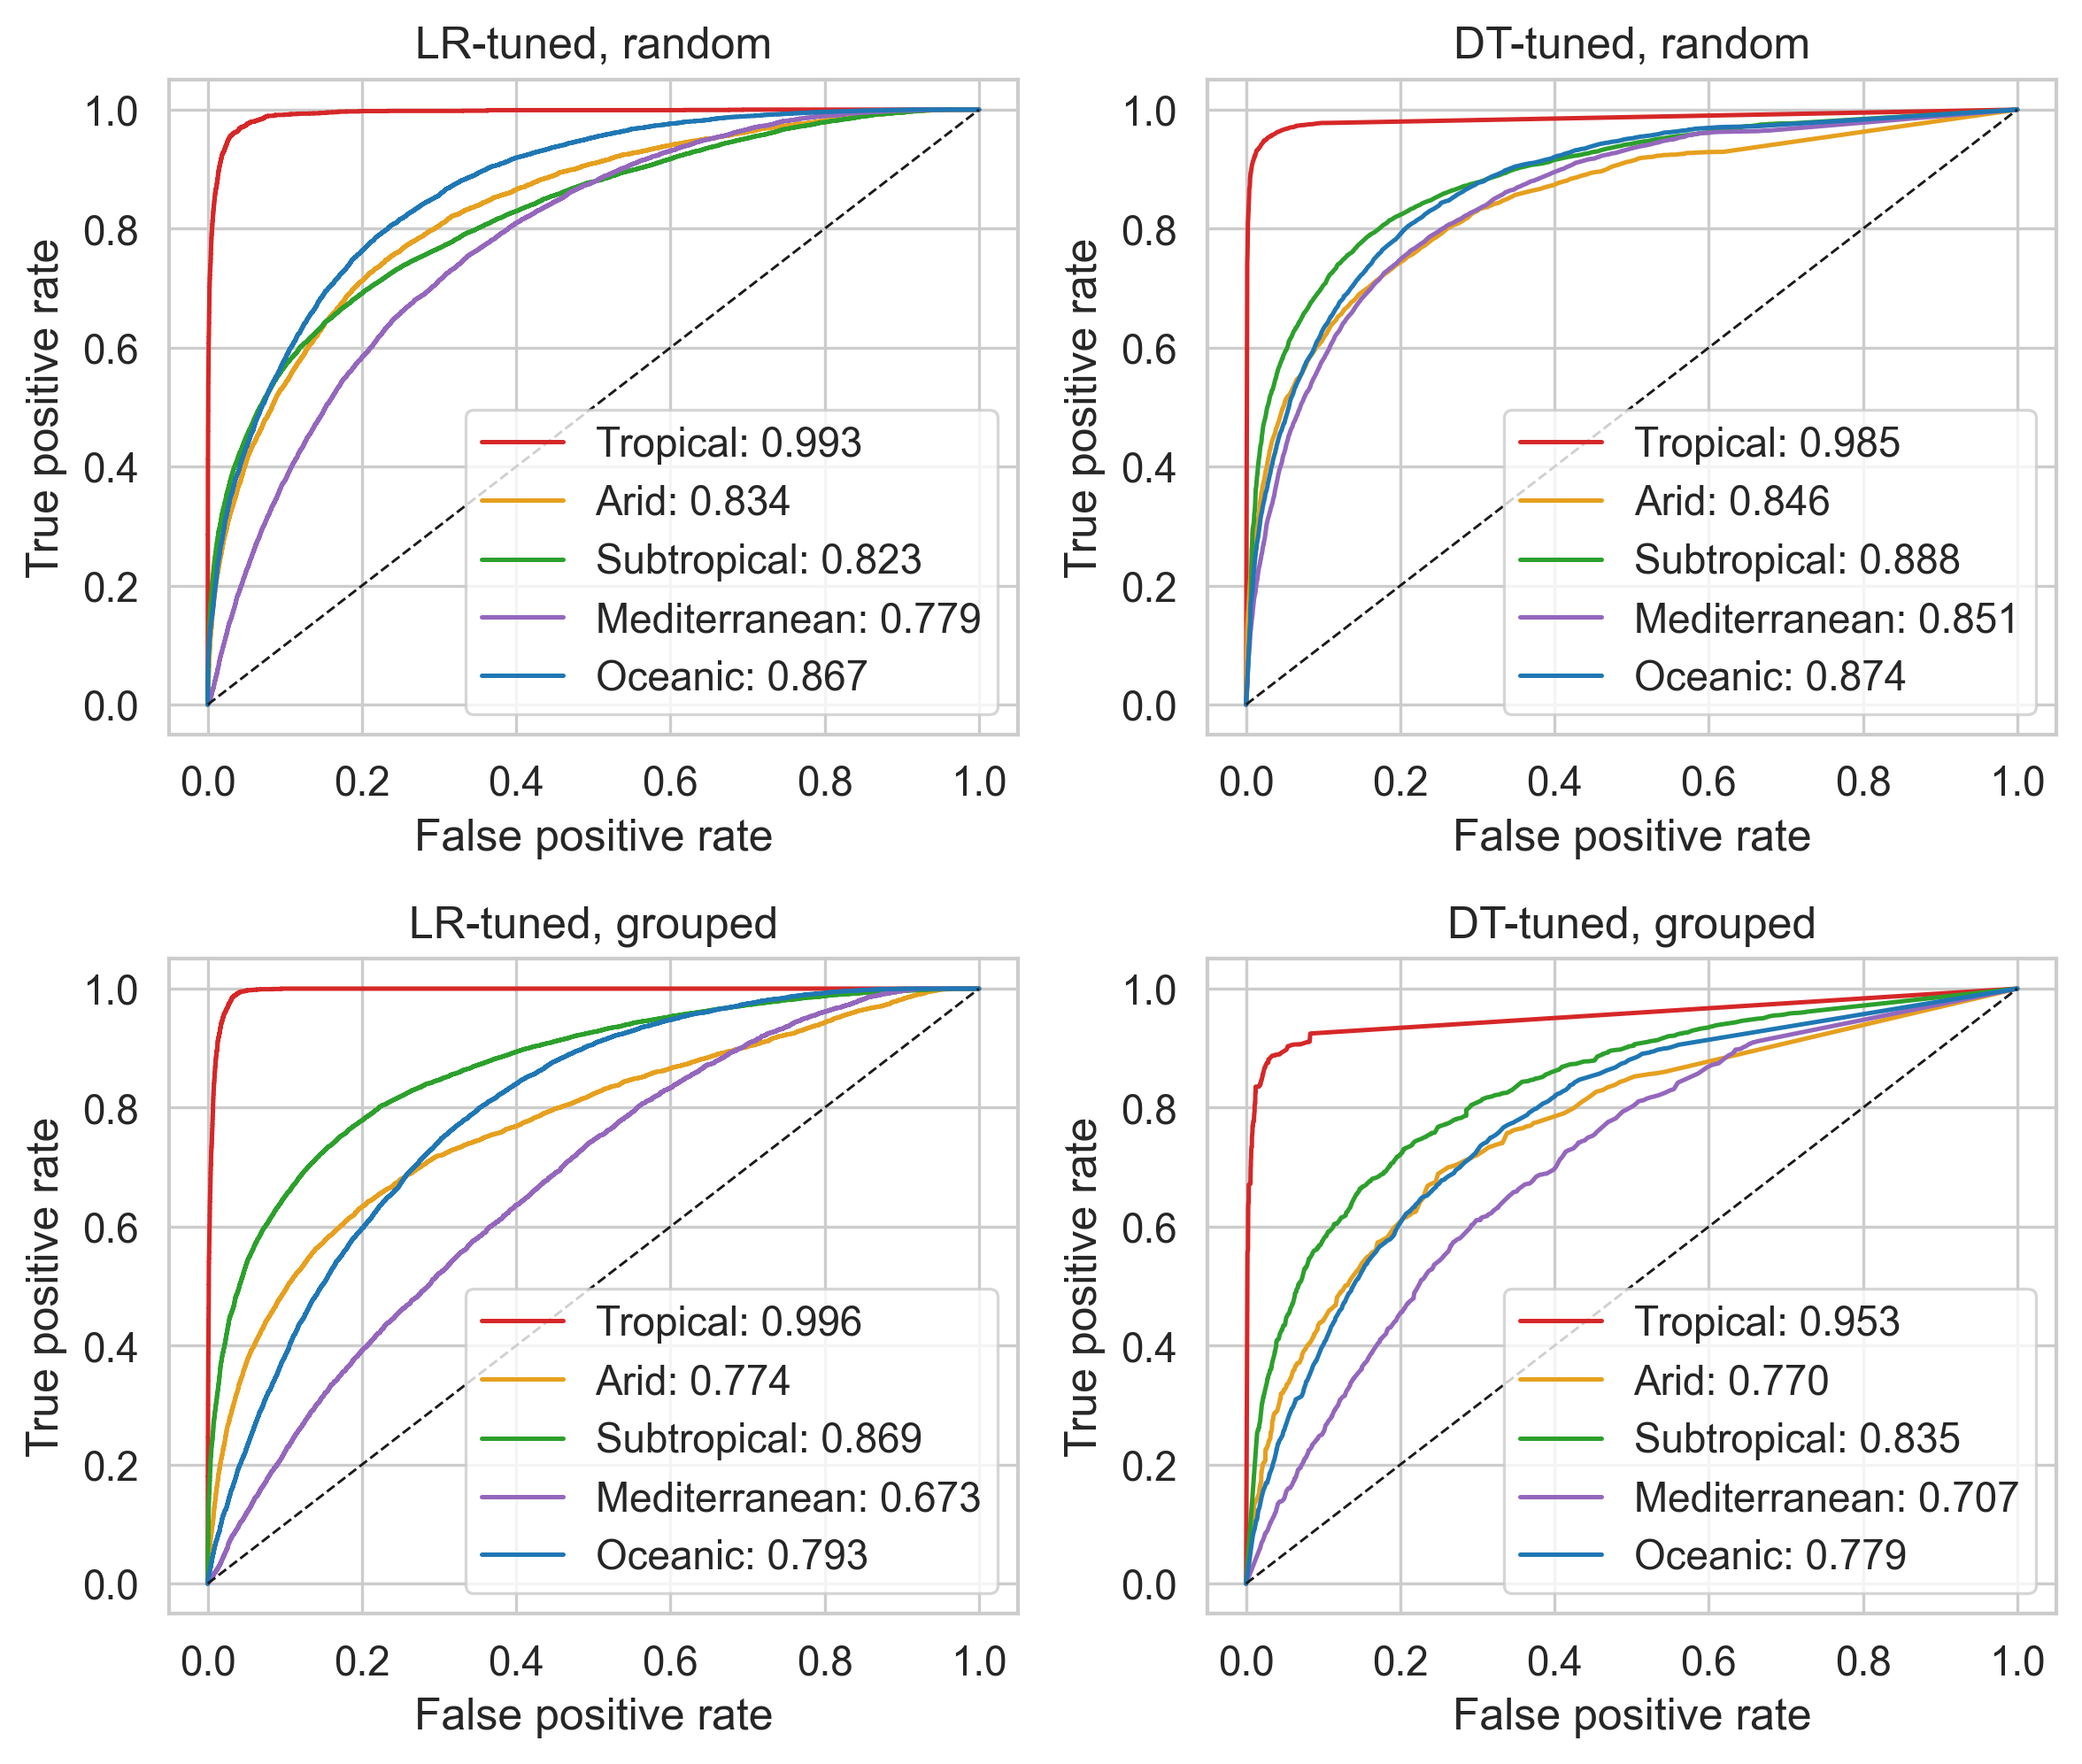
\includegraphics[width=\linewidth]{report_roc}
\caption{Training-only tuned LR and tree, shown on the historical random and grouped holdouts. These are course illustrations; primary generalisation results use nested OOF predictions.}\label{fig:roc}
\end{figure}

\textbf{Validation protocol.} All scorers use $F_1^{\rm macro}=\frac15\sum_{c=1}^5F_{1,c}$, with zero for undefined denominators. We stratify the table of stations into four outer folds, guaranteeing all five classes in training and test; inner three-fold station partitions cover all five classes as well. Assertions check both coverage and station disjointness. We do not reinterpret absent-class handling as a model-independent offset. Grid searches are rerun within every outer training fold. The primary score pools all OOF predictions; fold means are diagnostics, not interchangeable estimates. Seed 42 is the designated primary partition; seeds 0/7 reuse the same stations for sensitivity checks.

\textbf{Discussion (mandatory task).} @@DISCUSSION@@
\FloatBarrier

\section{Open-ended exploration}
\subsection{Model complexity, regularisation and protocol sensitivity}
We compare fixed LR, tuned LR/tree, degree-two polynomial LR (PolyLR) with stronger L2 regularisation, $k$-nearest neighbours ($k$NN), random forest (RF), a multilayer perceptron (MLP), fixed HGB and tuned HGB \citep{rf,boost}. The daily comparison starts from the same 20 inputs; polynomial LR expands them to 230 terms with $C=0.1$, versus $C=1$ for fixed linear LR. Subsequent history experiments change the available inputs. Table~\ref{tab:models} reports a common fixed-five metric for random, chronological and primary grouped evaluation. Time testing starts 2015-01-15 after training before 2015-01-01 (14-day gap). Time-protocol tuning uses forward validation within that training period. Random-protocol tuning uses training-only stratified folds.

The fixed $k$NN uses 15 neighbours; RF uses 200 trees with minimum leaf size 5; MLP uses hidden layers $(64,32)$ and L2 parameter $10^{-3}$. Fixed HGB uses learning rate 0.1 and at most 31 leaves. Other defaults follow the pinned scikit-learn version.

@@MODEL_TABLE@@
Seed 42 gives the highest score of the three partitions for all nine daily configurations. Its favourable results must therefore be read alongside the repeat means and ranges in Table~\ref{tab:models}; these repeats are not new independent evidence.

Polynomial LR reaches \DailyPoly\ versus \DailyLR\ for linear LR, a substantial point-estimate gain. This comparison changes polynomial features and regularisation together. In contrast, tuning HGB changes its score from \DailyHGB\ to \TunedHGB. Thus the tested increases in flexibility have unequal returns; a small tuning gain is not evidence that all useful information has been exhausted.
All candidates, including RF and MLP, receive all three protocols and repeated station folds. MLP has a 500-epoch cap and training-only row-based early stopping using validation accuracy; this internal criterion differs from the reported macro-F1. A reversible integer-label wrapper avoids a scikit-learn 1.7.2 string-label bug. Its \MlpFitCount\ fits take \MlpIterationRange\ epochs, with warnings in \MlpWarningFits\ fits; stopping is not proof of global optimisation. HGB early stopping is disabled, with 100 iterations. Nested HGB search varies learning rate, leaves and L2 over eight configurations. Limited search gains concern this budget, not an ultimate bottleneck. Selected parameters and diagnostics are in \texttt{results/fit\_audit.csv}.

Daily HGB's primary difference from RF is \HgbRfDifference\ (conditional 95\% interval \HgbRfInterval), and from MLP is \HgbMlpDifference\ (\HgbMlpInterval). We therefore distinguish a point-estimate ranking from evidence of meaningful superiority. The highest daily point estimate in this run belongs to \BestDailyName\ (\BestDailyScore); it is selected after comparison and has no new external test. Fixed HGB remains the predefined reference for history experiments. Different protocol scores describe different test populations; their differences do not causally partition temporal dependence and station recognition.

\subsection{History versus model flexibility}
For each station and day, we replace each of 18 daily features by a trailing mean, keeping two day-of-year features:
\[
\bar x^{(N)}_{s,t,j}=|W|^{-1}\sum_{\tau\in W}x_{s,\tau,j},\quad
W=\{\tau:t-N<\tau\le t,\ x_{s,\tau,j}\ \text{observed}\}.
\]
A feature is missing when fewer than $\max(1,\lfloor N/3\rfloor)$ observations are available. Thus 14 calendar days can mean only four valid readings for a variable. Rainfall means operate on log-transformed rainfall; vector means are net wind components. No future observations or labels enter the windows. With station-disjoint folds, calculating histories before the split does not cross the station boundary. Random day splits with overlapping histories answer a substantially easier, dependent-sample question.

Both LR and HGB are evaluated at fixed windows 1/3/7/14/30/90/365 days under all three station partitions (Fig.~\ref{fig:memory}). These curves compare configurations; their maximum does not establish an independently validated optimum. Separately, each outer fold selects a window by three-fold inner station CV and refits using only its outer training stations. LR's window-selection procedure obtains \SelectedWindowLR; HGB's obtains \SelectedWindow. The HGB--LR point-estimate gap narrows from \DailyModelGap\ with daily inputs to \HistoryModelGap\ with selected history. The chosen windows are recorded in Table~\ref{tab:windows}.

@@WINDOW_TABLE@@

\begin{figure}[htbp]\centering
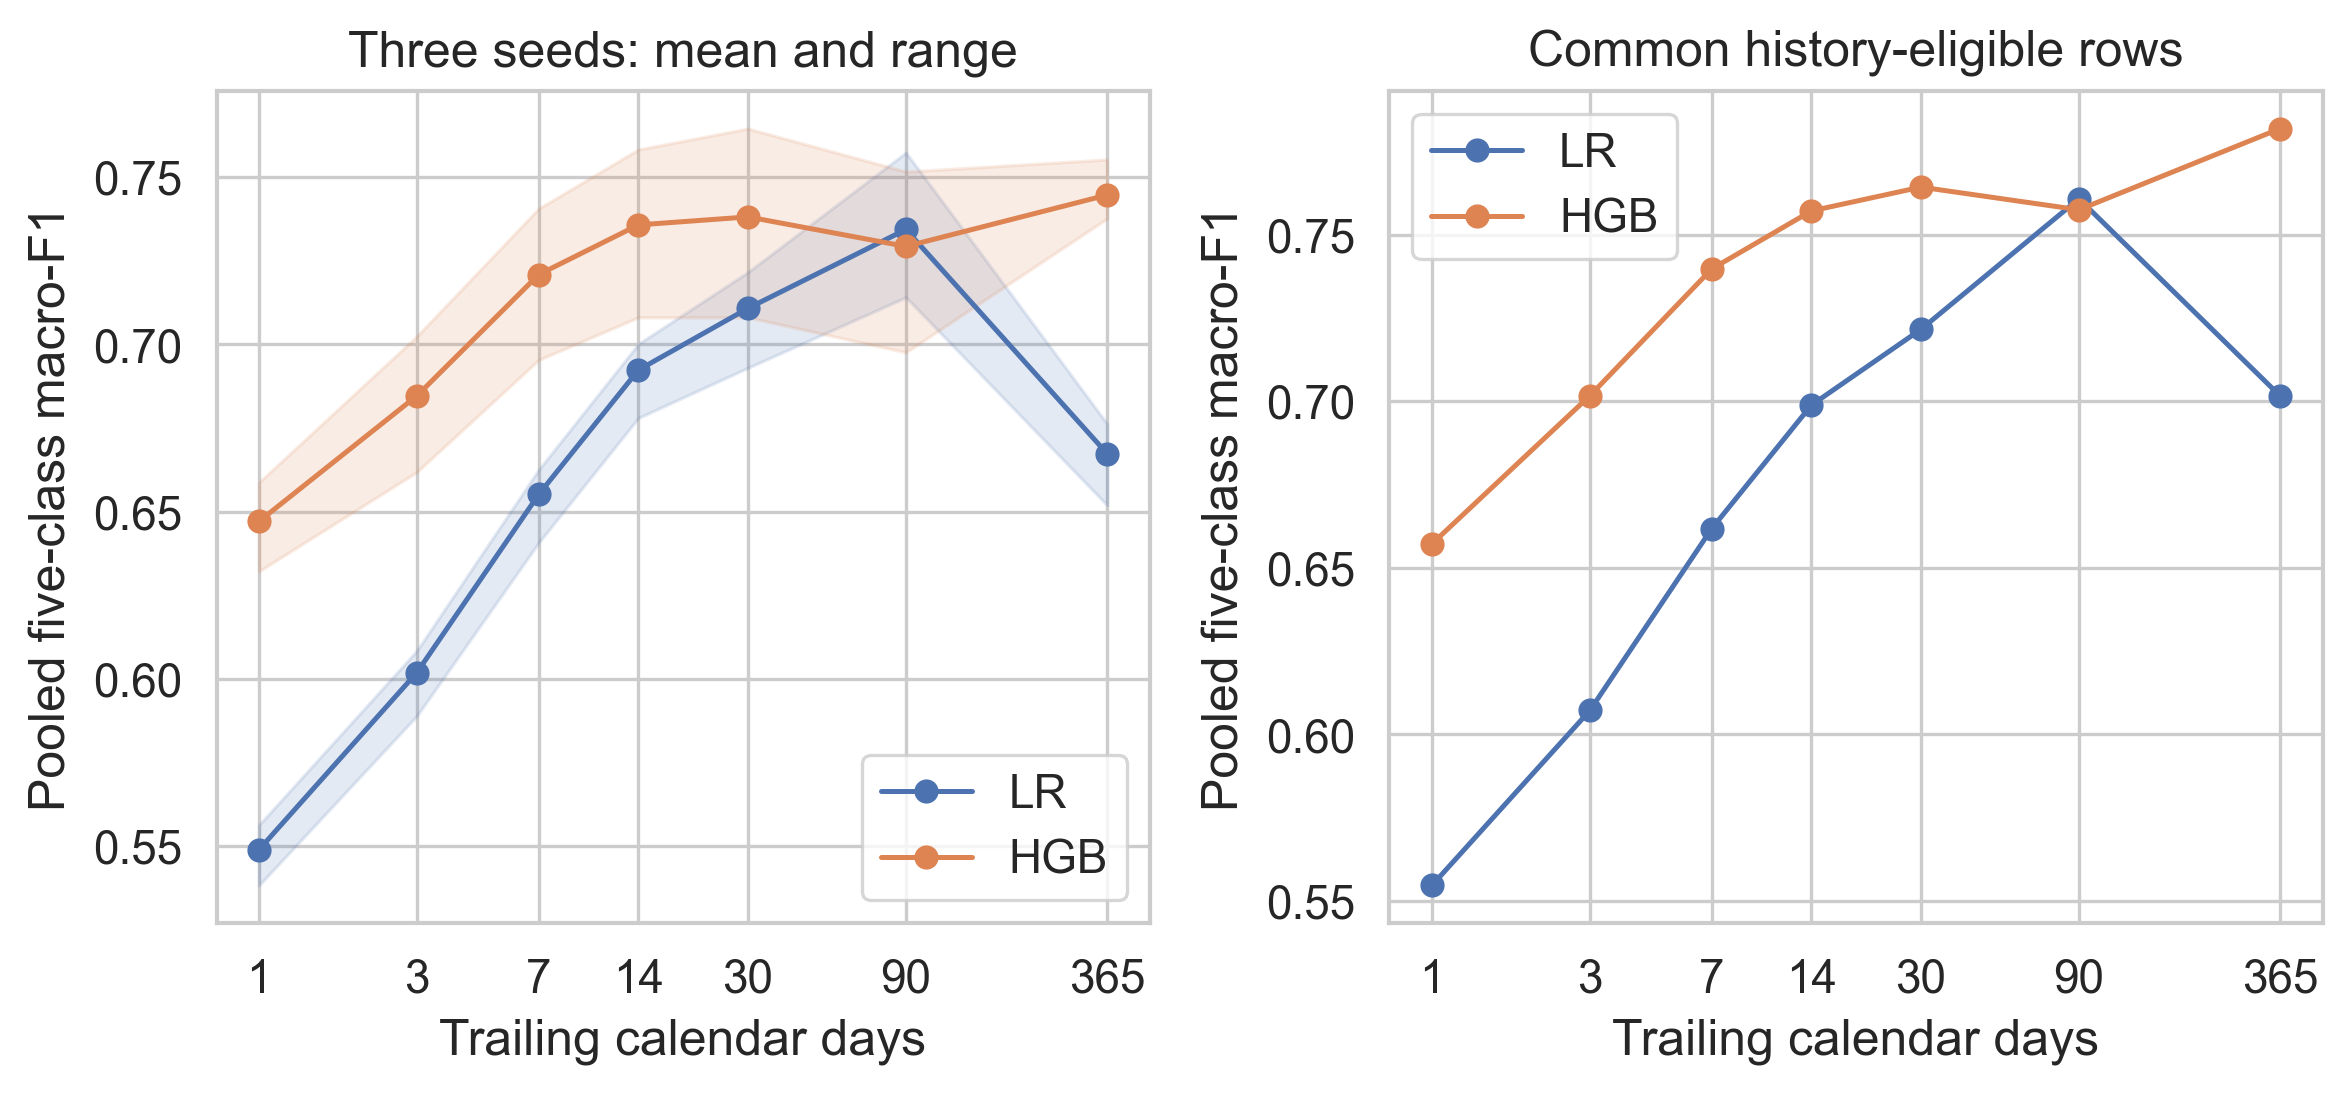
\includegraphics[width=\linewidth]{report_memory}
\caption{Model-by-window comparison. Left: mean/range across three reused-station partitions, not confidence intervals. Right: seed-42 OOF predictions evaluated on identical rows with at least 364 days since the station's first record.}\label{fig:memory}
\end{figure}

HGB's internally selected history procedure changes macro-F1 by \SelectedHistoryDifference\ relative to daily input (conditional paired interval \SelectedHistoryInterval). The fixed 14-day change is \HistoryDifference\ (\HistoryInterval). Window missingness and effective counts are exported.

On the common history-eligible rows, LR scores \CommonLRNinety/\CommonLRAnnual\ at 90/365 days; HGB scores \CommonHGBThirty/\CommonHGBAnnual\ at 30/365 days. The LR annual-window decline persists, while annual HGB becomes stronger on this subset. Excluding early records therefore matters, but does not explain both models in the same way. The restriction controls scoring rows, not training history, instrument availability or feature distributions. LR peaks at 90 days and falls at 365 days under all three partitions. HGB behaves differently: 30 days gives its highest primary fixed-window score, whereas 365 days gives its highest three-partition mean. There is no universal long-window collapse. These model-dependent patterns and the changing missingness weaken a single-mechanism explanation; neither 14 nor 365 days is established as a universal optimum.

\FloatBarrier
\subsection{Training-only feature selection and conditional uncertainty}
The multi-scale input contains 74 features (daily plus 7/30/90-day means). Within each outer training set, three disjoint class-covered station subsets A/B/C are used: train the importance model on A, rank by permutation loss on B, choose $k\in\{3,5,10,20,40,74\}$ using fits on A+B and scores on C. Refit on all outer training stations with that ranking and chosen $k$, then evaluate the untouched outer test. This prevents the former test-label feedback. The internally selected procedure obtains \SelectedFeatures, versus \FullFeatures\ using all 74 features; fixed top-20 obtains \TopTwenty. The selected counts are \SelectedFeatureCounts\ in fold order. Thus this selection procedure underperforms using all features. Fixed top-40 scores \TopForty, but promoting it after inspecting outer scores would reintroduce test-driven selection. Small ranking/validation station sets and correlated features can make the procedure unstable; this is a limitation, not a demonstrated universal failure of feature selection. Importance is predictive reliance, not a causal wind/climate mechanism.

We also give station-balanced metrics (each station has equal total sample weight). For uncertainty, 2,000 paired bootstrap draws resample whole stations within each climate group, preserving their daily records. The intervals condition on the fitted primary OOF predictions and observed network; they exclude retraining/selection variation and do not remove spatial dependence. Repeated-fold standard deviation is not a confidence interval. Neither fold-win counts nor an interval spanning zero establish equivalence.

\subsection{Stress tests and scope}
Fixed HGB is compared under core, full-sensor and full-plus-indicator policies, with primary macro-F1 \CorePolicy/\FullPolicy/\IndicatorPolicy. These are sensitivity comparisons, not test-driven policy selection. A 100-km exclusion buffer removes training stations close to each outer test group; the pooled score is \SpatialScore\ on \SpatialRows\ supported rows. The buffer also changes training size/composition, so any degradation is not a pure estimate of spatial dependence. All four folds remain class-covered; training coverage falls from 36 to \BufferedStations\ stations per fold. The lower score makes the network-transfer limitation practically consequential.

The raster marks \BoundaryStations\ as a labelled boundary station. Excluding boundary stations yields \BoundaryExclude\ versus \BoundaryExcludeReference\ for the original fit on the same scored rows; changing their labels to a different mapped group found in neighbouring pixels yields \BoundaryAlternative. This is local annotation sensitivity using the same raster, not an independent-map validation. Both the manual station match and map reference period remain structural limits. Table~\ref{tab:classes} shows that Arid remains the hardest group for the selected-history model. Its three lowest station accuracies are \WorstStations. These failures show why a pooled score near 0.76 does not establish reliable performance at every site.
@@CLASS_TABLE@@
\FloatBarrier

\section{Conclusion}
The original question remains viable: short-term weather can be evaluated for its ability to recover long-term climate labels. The revised experiments separate exploratory pictures, fixed-configuration comparisons and complete training-only selection procedures. The daily HGB reference rises from \DailyHGB\ to \SelectedWindow\ with training-only history selection, while LR reaches \SelectedWindowLR. History narrows the point-estimate gap between these two model classes more than the tested HGB parameter search improves its daily score. The useful window depends on the model, station partition and history availability; the annual HGB result contradicts a universal long-window decline. These findings describe the given network and tested configurations.

Our evidence does not establish a uniquely optimal observation window, causal attribution of random/grouped gaps, or transfer to arbitrary Australian sites. Only four tropical stations are available, labels come from one manually matched raster, and all redesign followed earlier exploration. More independent stations and label sources would strengthen external validity.

\section*{Reproducibility}
All code and figures are in the self-contained executed notebook. Python \PythonVersion\ and exact dependencies are in \texttt{requirements\_XX\_TaskA.txt}. Code-cell, raw-data, annotation and environment hashes define cache identity; old cache files cannot be silently reused. The complete rerun records \CacheMisses\ computed cache entries and \CacheHits\ hits; t-SNE also bypasses caches during the fresh run. Predictions, fold membership, diagnostics and CSV tables are in \texttt{results/}. This report's numerical macros/tables are generated from those files by \texttt{tools/build\_report.py}. The raw CSV is unchanged.

\clearpage
\begin{thebibliography}{12}\small
\bibitem{kaggle} Kaggle user jsphyg. Rain in Australia, version 2. \url{https://www.kaggle.com/datasets/jsphyg/weather-dataset-rattle-package}.
\bibitem{bom} Bureau of Meteorology. Station list IDCJMC0014, downloaded 2026-11-09. Original archive and manual station crosswalk included in the project.
\bibitem{kgc} Bryant et al. \emph{kgc: Koeppen-Geiger Climatic Zones}. R package; Python port \texttt{kgcpy} 1.1.8. \url{https://github.com/cwru-sdle/kgcpy}.
\bibitem{rubel} Rubel et al. The climate of the European Alps: shift of very high resolution K\"oppen-Geiger climate zones 1800--2100. \emph{Meteorologische Zeitschrift}, 26:115--125, 2017. doi:10.1127/metz/2016/0816.
\bibitem{map} Rubel et al. World Maps of K\"oppen-Geiger climate classification, March 2017 version, reference period 1986--2010. \url{https://koeppen-geiger.vu-wien.ac.at/present.htm}.
\bibitem{sklearn} Pedregosa et al. Scikit-learn: Machine learning in Python. \emph{JMLR}, 12:2825--2830, 2011.
\bibitem{tsne} van der Maaten and Hinton. Visualizing data using t-SNE. \emph{JMLR}, 9:2579--2605, 2008.
\bibitem{sil} Rousseeuw. Silhouettes: a graphical aid to interpretation and validation of cluster analysis. \emph{J. Comput. Appl. Math.}, 20:53--65, 1987.
\bibitem{ari} Hubert and Arabie. Comparing partitions. \emph{Journal of Classification}, 2:193--218, 1985.
\bibitem{rf} Breiman. Random forests. \emph{Machine Learning}, 45:5--32, 2001.
\bibitem{boost} Friedman. Greedy function approximation: a gradient boosting machine. \emph{Annals of Statistics}, 29:1189--1232, 2001.
\end{thebibliography}
\section*{Credit}
Group ID, member names and contribution percentages must be supplied by the group. Earlier development used Claude; the review-driven redesign, implementation, rerun and report revision used OpenAI Codex. The group must review the results and complete its own contribution statement. Activities and verification are recorded in \texttt{AI\_LOG.md}; no personal contributions are fabricated.
\end{document}
